\subsection{Q1.4}
\subparagraph{Here, we need to build the method called $updateJacobian$ of the $kinematicModel$ class. As we can have the transformation matrix from the base to a given frame, we can compute the Jacobian matrix of the manipulator for the end-effector like below. So, we need to find the angular and linear parts of the Jacobian for either revolute and prismatic joints.  }


\[\mathbf{^0 J_{e/b}} = \begin{pmatrix}
        \mathbf{^0 J^A_{1}} & \mathbf{^0 J^A_{2}} &  ... & \mathbf{^0 J^A_{e}} \\
        \mathbf{^0 J^L_{e/1}} & \mathbf{^0 J^L_{e/2}} & ... & \mathbf{^0 J^L_{e/e}} \\
    \end{pmatrix}\]

\subsubsection{Angular Jacobian} 
\subparagraph{The Angular Jacobian for any revolute joint is the third column of the rotation matrix of the joint with respect to the base $^0\mathbf{K_i}$. On the other hand, for prismatic joints, it's a zero vector since there's no any angular velocity that can be generated from translation. So, we have : }
\[
^{0}\mathbf{J}{}^A_i = 
\begin{cases} 
^{0}\mathbf{K}_i & \text{if } \Gamma_i = R \\ 
\mathbf{0} & \text{if } \Gamma_i = P 
\end{cases}
\]

\subsubsection{Linear Jacobian} 
\subparagraph{The Linear Jacobian for any revolute joint is the cross product between $^0\mathbf{K_i}$ and, $\mathbf{r}_{e/i} = \mathbf{r}_{e} - \mathbf{r}_{i} $ which are:
\newline
$^0\mathbf{K_i}$ : the third column of the rotation matrix of the joint i with respect to the base.
\newline
$\mathbf{r}_{e}$ : a vector that represents the position of the end effector, with respect to base.
\newline
$\mathbf{r}_{i}$ : a vector that represents the position of the joint i with respect to base.
\newline
On the other hand, for prismatic joints, it's just $^0\mathbf{K_i}$. So we have : }
\[
{}^{0}\mathbf{J}{}^L_{e/i} = 
\begin{cases} 
\left( ^0\mathbf{K}_i \times (\mathbf{r}_{e} - \mathbf{r}_{i})  \right) & \text{if } \Gamma_i = R \\ 
^0\mathbf{K}_i & \text{if } \Gamma_i = P
\end{cases}
\]
\subsubsection{Initial Configuration}
\subparagraph{These are the initial joint parameters :}
\[
q_{init} = \begin{pmatrix}
    \frac{\pi}{4} & -\frac{\pi}{4} & 0 & -\frac{\pi}{4} & 0 & 0.15 & \frac{\pi}{4}
\end{pmatrix}
\]
\subparagraph{In the figures \ref{fig:Initial Configuration1} and \ref{fig:Initial Configuration2}, we can see the initial configuration of the robot with respect to the base frame. All joint positions are marked with circles.}

\begin{figure}[h!]
    \begin{minipage}{0.5\textwidth}
        \centering
        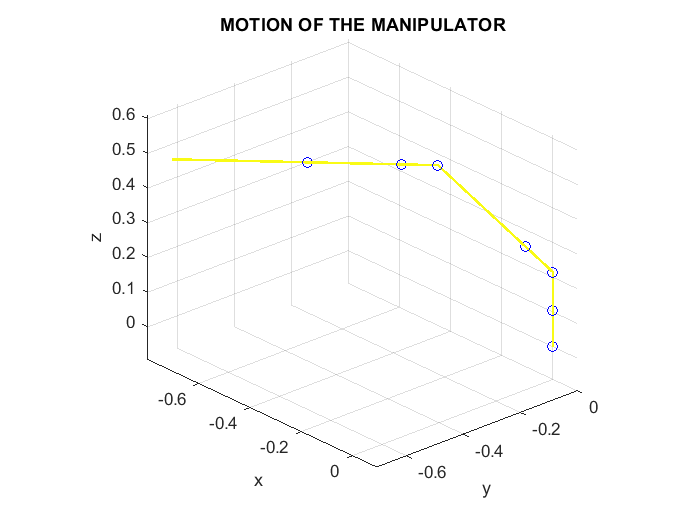
\includegraphics[width=\linewidth]{template_MCM_lab2_2024_25/Resources/q1.1.png}
        \caption{Isometric View of the Initial Configuration}
        \label{fig:Initial Configuration1}
    \end{minipage}%
    \hfill
    \begin{minipage}{0.5\textwidth}
        \centering
        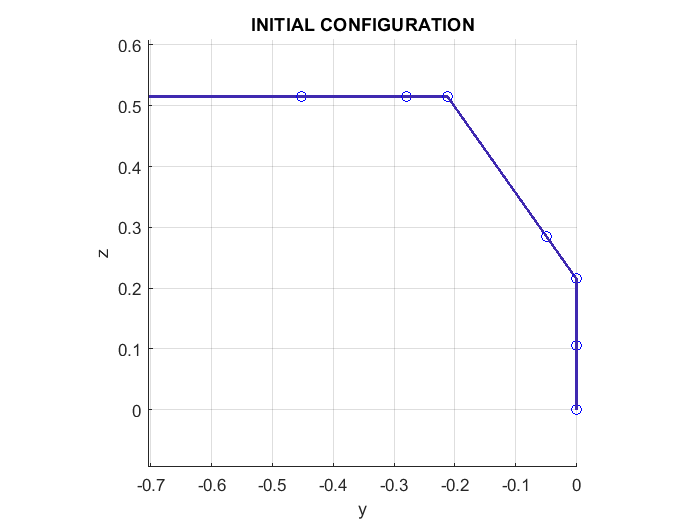
\includegraphics[width=\linewidth]{template_MCM_lab2_2024_25/Resources/q1.3.png}
        \caption{Side View of the Initial Configuration}
        \label{fig:Initial Configuration2}
    \end{minipage}
\end{figure}

\subsubsection{Final Configurations}
\subparagraph{These are the final joint parameters :}
\[
q_f = \begin{pmatrix}
    \frac{\pi}{4} + \frac{\pi}{6} & -\frac{\pi}{4} & 0 & -\frac{\pi}{4} & 0 & 0.15 & \frac{\pi}{4}
\end{pmatrix}
\]
\subparagraph{The robot transitions to a new configuration where the first joint has to rotate of $\pi/6$ around the $z_0$ axis. The remaining joints don't have rotations or translations from their initial configuration. So the motion of the robot is circular around the $z_0$ axis as we can see in the figure \ref{fig:Final Configuration1} in order to arrive in the final configuration as we can see in figure \ref{fig:Final Configuration2}}

\begin{figure}[h!]
    \begin{minipage}{0.5\textwidth}
        \centering
        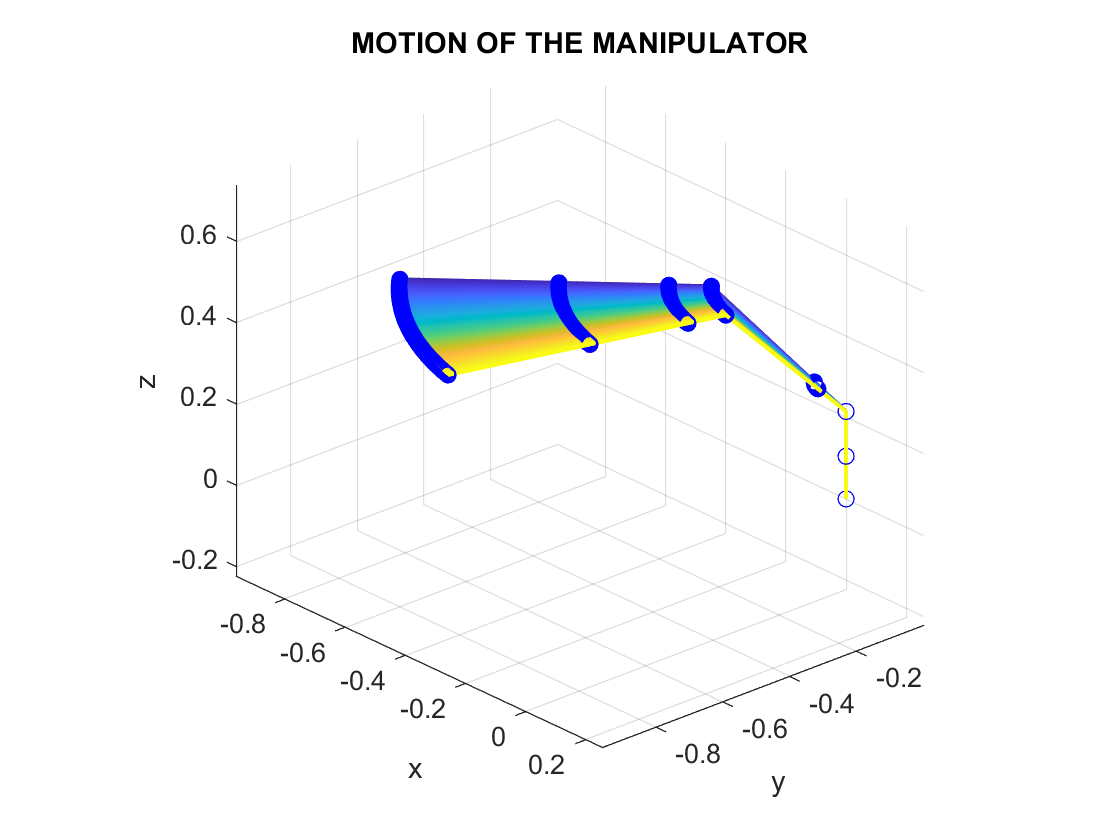
\includegraphics[width=\linewidth]{template_MCM_lab2_2024_25/Resources/motion_of_the_manipulator.png}
        \caption{Isometric View of the Final Configuration}
        \label{fig:Final Configuration1}
    \end{minipage}%
    \hfill
    \begin{minipage}{0.5\textwidth}
        \centering
        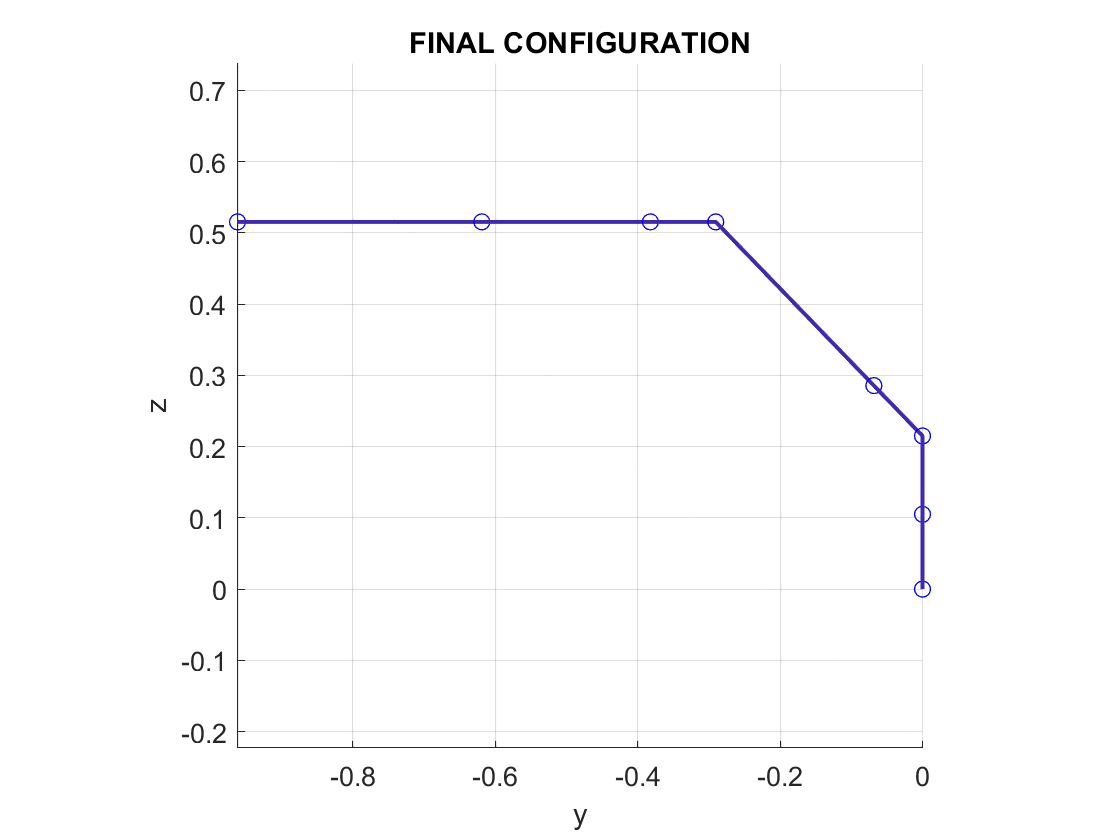
\includegraphics[width=\linewidth]{template_MCM_lab2_2024_25/Resources/final_configuration.png}
        \caption{Side View of the Final Configuration}
        \label{fig:Final Configuration2}
    \end{minipage}
\end{figure}

\subsubsection{Jacobian}
\subparagraph{
The Jacobian matrix, J(q) gives the relationship between joint velocities and the end-effector's linear and angular velocities. The Matlab function $kinematicModel$ gives us this Jacobian matrix for the robot with $q_{init}$ :
}

\[J(q_{init}) = \begin{pmatrix}
        0 & -0.7071 & -0.5 & -0.7071 & -0.7071 & 0 & -0.7071 \\
        0 & 0.7071 & -0.5 & 0.7071 & -0.7071 & 0 & -0.7071 \\
        1 & 0 & 0.7071 & 0 & 0 & 0 & 0 &  \\
        0.7039 & 0.2125 & 0.3475 & 0 & 0 & -0.7071 & 0 \\
        -0.7039 & 0.2125 & -0.3475 & 0 & 0 & -0.7071 & 0 \\
        0 & 0.9955 & 0 & 0.6950 & 0 & 0 & 0 \\
    \end{pmatrix}\]

% TODO : Comment the rank and the result, can be commandable because Xp = J q

\subparagraph{The Jacobian matrix is rank 6, indicating 6 linearly independent rows or columns. This suggests the manipulator has 6 degrees of freedom (DOF) in its task space, allowing full control over the end-effector's linear and angular velocities. Since the matrix has more columns than rows, there may be one redundant degree of freedom, possibly due to passive or redundant joints. With this Jacobian matrix $J(q_{init})$, we could compute the end-effector's linear and angular velocities near the initial state.}

% Add bTe of the final pose ? 